\documentclass[12pt,twoside,openright]{ociamthesis}  % default square logo 
%\documentclass[12pt,beltcrest]{ociamthesis} % use old belt crest logo
%\documentclass[12pt,shieldcrest]{ociamthesis} % use older shield crest logo

%load any additional packages
\usepackage{amssymb}
\usepackage{nomencl}
\usepackage{graphicx}
\usepackage[table,xcdraw]{xcolor}
\usepackage{algorithm}
\usepackage{algorithmic}
\usepackage{caption}
\usepackage{fancyhdr}
\usepackage{emptypage}
\usepackage{hyperref}
\usepackage{abntex2cite}
\usepackage{listings} % for code snippets
\usepackage[utf8]{inputenc}
\usepackage[french, american]{babel}
\usepackage{afterpage}
\usepackage[T1]{fontenc}

 %remove headers and footers from empty pages
%input macros (i.e. write your own macros file called mymacros.tex 
%and uncomment the next line)
%\include{mymacros}

\setlength{\headheight}{14.5pt} %suppress warning

\title{An Architecture for Task and Traffic Offloading in Edge Computing via Deep Learning\\[1ex]     %your thesis title,
}   %note \\[1ex] is a line break in the title

\author{Alessandro Gaballo}             %your name
%\college{Politecnico di Torino}  %your college
\college{EURECOM - Data Science and Engineering}  %your college

%\renewcommand{\submittedtext}{change the default text here if needed}
\degree{Research carried out at Saint Louis University under the supervision of Dr. Flavio Esposito}     %the degree
\degreedate{January 2018}         %the degree date

\newcommand{\itab}[1]{\hspace{0em}\rlap{#1}}
\newcommand{\tab}[1]{\hspace{.2\textwidth}\rlap{#1}}
\makenomenclature
%end the preamble and start the document
\begin{document}
\pagenumbering{gobble} 
%this baselineskip gives sufficient line spacing for an examiner to easily
%markup the thesis with comments
\baselineskip=18pt plus1pt

%set the number of sectioning levels that get number and appear in the contents
\setcounter{secnumdepth}{3}
\setcounter{tocdepth}{3}


\maketitle                  % create a title page from the preamble info
%!TEX root = tesi.tex
\cleardoublepage
\begin{citazioni}
\begin{flushright}
\textit{This thesis is dedicated to my parents,\\who taught me the value of respect and unconditionally believed in me, giving me\\the support and the strength I needed.\\From the bottom of my hearth, thank you.}
\end{flushright}
\end{citazioni}        % include a dedication.tex file
\include{acknowlegements}   % include an acknowledgements.tex file
\begin{abstract}
The spreading of smart mobile devices and the development of IoT has brought computation power in everyone's pocket, allowing people to perform simple task with their smartphones. There are some tasks however, which are more computationally expensive and therefore cannot be performed on a mobile device; for these type of tasks computation offloading represents a valid solution. Computation offloading is the process of transferring computation tasks to another platform for reasons such as limited computation resources and energy saving, which are evident in mobile and IoT devices. Typically, tasks are offloaded to powerful machines in the cloud, however for time sensitive applications the cloud could be too far, this is why the edge computing paradigm is spreading. Edge computing moves the processing from the core to the edge of the network, improving user experience by reducing the perceived latency. One way to reduce latency is to chose a proper path to the destination; paths advertised by the routing algorithms are not always the best because they don't take into account the network conditions. Our conjecture is that cooperative routing-based methods will steer edge traffic with (statistically) better quality, i.e., shorter end-to-end delays than reaction-based methods, such as Cartographer \cite{facebook_LB}. A way to perform path prediction is to use machine learning techniques, which in the last few years have spreaded and changed the way software is made~\cite{karpathy}. Machine learning is the field of computer science that gives computers the ability to learn without being explicitly programmed~\cite{5392560}, by extracting patterns from data. Recently, many goal have been achieved with the use of machine learning in the field of computer vision, gaming, text and speech recognition, but not much has been done in networking: this work is a first approach to machine learning in networking for path prediction. In this project, we present a system architecture to manage the offloading process of a task at the edge of the network: this architecture has a modular design so that the offloading policies could be easily plugged into the system. As part of the offloading policies we implement a path prediction system based on a deep neural network, with the aim of reducing the latency with respect to the standard routing policies. The proposed system performs better than the traditional routing policies in terms of latency, throughput and signaling overhead.
\end{abstract}          % include the abstract
\begin{otherlanguage}{french}
\begin{abstract}
La diffusion d’appareil mobiles intelligents et le développement de l’Internet des Objets a amené la puissance de calcul dans les poches de tout le monde, permettant aux personnes d’effectuer des tâches simples grâce à leurs smartphones. Il existe cependant certaines tâches qui demandent plus de puissance de calcul et ne pouvant donc pas être effectuées sur des appareils mobiles (e.g., une flotte de drones capturant des images multicouches devant être traitées avec des opérations de machine learning telles que la reconnaissance de plaques d’immatriculation or de visages); pour ces applications en temps réel, la délocalisation de calculs représente une solution viable.

Le processus de délocalisation de calculs consiste en la délégation de tâches complexes à des serveurs situés à la périphérie du réseau. Il est utile pour minimiser les temps de réponse ou la consommation d’énergie, des contraintes critiques pour les appareils mobiles et les objets connectés. Délocaliser de telles tâches au cloud est inefficace étant donné que l’infrastructure des serveurs de cloud sont trop distantes des objets connectés. Le Edge Computing (ou calcul de périphérie) déplace le calcul du cœur à la périphérie du réseau, améliorant l’expérience de l’utilisateur en réduisant les temps de latence perçus. Un des mécanismes fondamentaux pour réduire les temps de latence grâce au edge computing est de choisir un chemin adéquat jusqu’à la destination; les algorithmes de recherche du plus court chemin communément utilisés sont agnostiques face à la performance (et donc aux temps de latence): ils ne prennent pas en considération les conditions du réseau. Une des hypothèses que nous validons dans cette publication est que les méthodes basées sur le routage coopératif peuvent diriger (i.e. acheminer ou transmettre) le trafic de périphérie avec des délais bout-en-bout (statistiquement) plus courts que des méthodes basées sur la réaction, telles que les répartiteurs de charge~\cite{facebook_LB}.

Pour prédire les métriques de chemin, nous utilisons des techniques de machine learning, qui ont beaucoup impacté la manière dont nous développons du logiciel ces dernières années~\cite{karpathy}. En particulier, dans ce projet, nous présentons une architecture pour l’orchestration de la délocalisation périphérique: le design de l’architecture est modulaire de manière à ce que les politiques de délocalisation puissent être facilement adjointes au système. Une politique efficace de prédiction de chemin pour les mécanismes de délocalisation que nous avons implémentée est le Long Short Term Memory (LSTM), une approche de Deep Learning. Notre évaluation de performances montre que notre méthode fonctionne mieux que les politiques traditionnelles de routage en termes de surcharge de débit de données. 

\end{abstract}
\end{otherlanguage}          % include the abstract
\pagestyle{fancy}
\renewcommand\chaptermark[1]{\markboth{\thechapter\ #1}{}}
\fancyhf{}

\fancyhead[LE,RO]{\bfseries\leftmark}
\fancyhead[RE,LO]{\rightmark}
\begin{romanpages}          % start roman page numbering
\tableofcontents            % generate and include a table of contents
\listoffigures              % generate and include a list of figures
\listoftables
\printnomenclature[3cm]
\end{romanpages}% end roman page numbering
\pagenumbering{arabic}
\afterpage{\cfoot{\thepage}} %start regular page numbering
%now include the files of latex for each of the chapters etc
\chapter{Introduction}

%\section{Overview}
Data-intensive computing requires seamless processing power which is often not available at the network-edge but rather hosted in the cloud platforms. The huge amount of mobile and IoT devices that has become available in the past few years, is able to produce a massive quantity of data, which contributes to the very famous world of big data. The majority of these devices do not have or can not handle the computational requirements to process the data they capture and so leave to the cloud the responsibility to perform the computations. This process of transferring computation tasks to another platform is called {\it computation offloading} and it is crucial to the mobile devices because it results in lower processing time and energy consumption. In critical scenarios, such as natural disasters, not only computation offloading becomes necessary, but latency requirements become more strict, making paths management essential to satisfy these requisites. Current systems for traffic offloading are usually performance unaware (e.g. OSPF, ECMP), achieving therefore sub-optimal performance. Many people have proposed the use of machine learning techniques to solve network problems, including traffic classification~\cite{nguyen2008survey} and latency prediction~\cite{end-to-end}; however, no one has ever used LSTM to train network devices to steer traffic in a virtual network. In this work we develop an architecture to be deployed at the edge of the network to assist the offloading process and make use of machine learning techniques to perform path management. The goal is to outperform the classic routing policies in terms of latency and throughput by learning implicit patterns in network traces.

In particular, in this thesis we make the following contributions:
\begin{itemize}
\item the design of an edge computing architecture for \textbf{offloading} management in edge computing, that describes the macro blocks required for such a system and proposes an offloading protocol
\item a deep learning based \textbf{path prediction system} as part of the offloading architecture; this system is meant to be used as an offloading policy in the proposed architecture 
\item performance evaluation extended to different use cases: we evaluate the prediction system first for its ability to learn from an existing model, second as a routing algorithm replacement.
\end{itemize}
%\section{Structure}
This report is organized as follows:
\paragraph{Chapter~\ref{ch:background}} contains a brief background about machine learning and networking notions and main techniques used in this project.
\paragraph{Chapter~\ref{ch:contribution}} describes the personal contribution of this project, including the details about the architecture and the implementation of the path predictor system.
\paragraph{Chapter~\ref{ch:related_work}} illustrates a summary of the related work.
\paragraph{Chapter~\ref{ch:results}} shows considerations and results of the implemented system.
\paragraph{Chapter~\ref{ch:conclusion}} presents comments about the outcome of the project and possible future developments.


\chapter{Background}
\label{ch:background}
Before describing our approach, we would like to give a brief introduction to some of the methods and concepts that are needed to understand our implementation and related work. Specifically, we first shortly describe the network technologies required to understand the aim of this project; next, we give an introduction about machine learning and its applications. Even though these might seem separate topics,  keep in mind that in this project, we take advantage of machine learning to address networking problems.

\section{Software-Defined Networking}
Software-Defined Networking (SDN) is paradigm that promises to break networks' vertical integration of control and data plan, separating the network's control logic from the underlying routers and switches, promoting (logical)  centralization  of  network  control,  and  introducing  the ability  to  program  the  network.  The  separation  of  concerns introduced   between   the   definition   of   network   policies,   their implementation  in  switching  hardware,  and  the  forwarding  of traffic, is key to the desired flexibility: by breaking the network control  problem  into  tractable  pieces,  SDN  makes  it  easier  to create and introduce new abstractions in networking, simplifying network  management  and  facilitating  network  evolution~\cite{kreutz2015software}.SDN is a network architecture built on four principles:
\begin{enumerate}
\item separate control and data planes: network devices are left responsible only of packet forwarding
\item flow-based forwarding: packets are forwarded by looking to a set of fields instead of only the destination, introducing great flexibility~\cite{mckeown2008openflow}
\item external control logic: the control logic is moved to an external entity called SDN controller or Network Operating System, that is a software platform that provides abstractions to facilitate the programming of forwarding devices
\item programmable network: software running on top of the NOS allows to program the network; this is considered the main value of SDN.
\end{enumerate}
SDN has successfully opened the way towards a next generation networking, creating an innovative research
and  development  environment,  promoting  advances  in  switch  and  controller platform design,  evolution of performance  of  devices  and  architectures, security and dependability.

\section{Knowledge-Defined Networking}
Knowledge-defined networking (KDN)~\cite{mestres2017knowledge} is a new paradigm that promotes the application of Artificial Intelligence (AI) to control and operate networks thanks to the rise of SDN. SDN provides a centralize control plane, a logical single point with knowledge of the network; moreover, current network devices have improved computing capabilities, which allow them to perform monitoring operations commonly referred to as network telemetry~\cite{kim2015band}. Information provided by network telemetry are usually provided to a centralized Network Analytics (NA) platform~\cite{clemm2015dna}, that combined with SDN can bring to light the Knowledge Plane proposed in~\cite{clark2003knowledge}. Knowledge-Defined Networking is the paradigm resulting from the combination of these tools, specifically Software Defined Networking, Network Analytics and Knowledge Plan. In the KDN paradigm, the knowledge plane has a rich view of the network; this view is transformed into knowledge via Machine Learning (ML) and used to make decisions. The ultimate goal of KDN is to combined SDN, NA and ML to provide automated network control.
%
%\section{Routing}
In networking, routing is the process of selecting a path in or between networks. Routing directs network packets from their source toward their destination through intermediate network nodes by specific packet forwarding mechanisms. Forwarding is performed on the basis of routing tables, which maintain a record of the routes to various network destinations. Thus, constructing routing tables, is very important for efficient routing.Dynamic routing constructs routing tables automatically thanks to the information carried by the routing protocols, that are usually classified in \textit{distance vector} and \textit{link-state} algorithms.

%\paragraph{BGP} (Border Gateway Protocol) is a protocol designed to exchange routing and reachability information among or within autonomous systems. In this second application it is also referred to as Internal BGP, or iBGP. In contrast, the Internet application of the protocol may be referred to as External BGP, or eBGP. BGP is typically used by Internet Service Providers (ISP) to establish routing between one another, or in large private networks to join a number of large Open Shortest Path First (OSPF) networks, when OSPF by itself does not scale to the size required. Routing informations are exchanged between neighbors called peers; in order to communicate, these peers require a manual configuration.

\paragraph{OSPF} is a link-state routing algorithm for IP networks. OSPF falls in the family of iBGP and it is widely adopted in large networks. It works thanks to a map of the network, built by gathering link state information from available routers. The maps is used to compute the shortest-path tree for each route using a method based on Dijkstra's algorithm. The OSPF routing policies are dictated by link metrics associated with each routing interface, typically the interface speed.

%\section{Machine Learning}
Machine learning is a field of computer science that studies the ability of making computers learn without explicitly programming them~\cite{5392560}. In machine learning there are three main approaches: supervised learning, unsupervised learning and reinforcement learning. Supervised learning is used to classify labeled data, the label is a sort of supervisor describing the class of an observation. In unsupervised learning on the other hand there is no supervisor, meaning that data are unlabeled and the goal is to find the hidden relation of the data. Reinforcement learning is learning what actions to do so as to maximize a numerical reward signal without being told which actions to take but instead discovering which yield the most reward by trying them \cite{Sutton98reinforcementlearning}. Among the several branches of machine learning, neural networks and in particular deep learning, have recently attracted a lot of attentions.

%\subsection{Deep Learning}
Teaching a computer to solve tasks that are hard to describe formally (e.g. speech recognition) is challenging; the solution is to allow computers to learn from experience and understand the world in terms of a hierarchy of concepts, with each concept defined through its relation to simpler concepts. The hierarchy of concepts enables the computer to learn complicated concepts by building them out of simpler ones. If we draw a graph showing how these concepts are built on top of each other, the graph is deep, with many layers. For this reason, we call this approach to AI deep learning~\cite{Goodfellow-et-al-2016}. In other words, deep learning can be described as the set of machine learning techniques that concatenate multiple layers of processing units (typically non-linear), for feature extraction and transformation  ~\cite{deep_learning_heterogeneus}. The first working deep learning algorithm was a multilayer perceptrons developed by Ivakhnenko et al.~\cite{ivakhnenko1973cybernetic}. Later on new techniques including Convolutional Neural Networks (CNNs) and Recurrent Neural Networks (RNNs) were developed; these techniques dramatically increased AI performance in tasks such as image recognition. More recently deep learning has been used to build AlphaGo~\cite{alphago}, a program that plays the board game Go and managed to beat, in 2017, the Go world No.1 Ke Jie.

\section{LSTM}
Long Short-Term Memory cells are a further development of Recurrent Neural Networks (RNNs). They were developed by Hochreiter and Schmidhuber in 1997 and have been further improved ever since~\cite{Greff2016}. The major flaw of a traditional neural network is that it does not capture the relation between the input it currently looks at and the previous training example. This however, is crucial for e.g. developing a language model. Making predictions about a subsequent word strongly depends on the preceding words. RNNs try to solve this problem; yet it turns out that they are not scalable to model long-term dependencies in practice. This is due to numerical problems commonly referred to as the \textit{vanishing/exploding gradient} when weight updates are backpropagated through the time steps. LSTMs overcome this problem and enable capturing long-term temporal dependencies among the input elements. They are considered state-of-the-art in numerous sequential prediction tasks such as Speech Recognition, Handwriting Recognition, Language Translation and many others.

The novelty of LSTMs compared to conventional RNNs is the introduction of the \textit{LSTM cell}. Figure \ref{fig:lstm} gives an overview over such a cell that is repeated three times, each receiving the current input as well as the output of the previous cell. For instance, the prediction $h_{t+1}$ (through feedforward) is based on the corresponding input $x_{t+1}$ as well as on the output of the previous cell. The LSTM cell is responsible for maintaining and updating a state that keeps track of the input that has been processed over time. Which information precisely should be kept and which overwritten is decided based on the training of the network. Each cell has associated weights that are updated during each backward pass such that the cell keeps the information that optimizes predictions. The major advantage of introducing this cell is that the \textit{Backpropagation Through Time} does not need to flow through numerous activation gates between the hidden layers. The transfer from cell to cell only flows through pointwise multiplications and additions. This way the numerical problems of RNNs are avoided.

\begin{figure}
\centering
\includegraphics[width=0.75\textwidth]{img/lstm}
\caption{LSTM cell overview.\protect\footnotemark}
\label{fig:lstm}
\end{figure}
\footnotetext{Taken from colah's blog: http://colah.github.io/posts/2015-08-Understanding-LSTMs/}


\chapter{Contribution}
The contributions produced by this project are:
\begin{itemize}
\item an \textbf{offloading system} conceived as a general architecture to be used in edge computing
\item a \textbf{path prediction system} that can be plugged into the offloading architecture and extended to different use cases
\end{itemize}

\section{Offloading System}
Edge computing is a recent computing paradigm that is trying to push data processing at the edge of the network, where the data is being generated. The goal is to reduce communication costs by keeping the computing close to the source of data. At the best of my knowledge, there hasn't been any effort in trying to implement a general abstraction - like the ISO/OSI stack (figure \ref{fig:iso_stack}) - which provides the guidelines for the protocol implementations. The proposed system is a first draft of how such abstraction could be implemented with all the limitations of a six-months work.
\begin{figure}[ht]
\includegraphics[width=\textwidth]{img/osi}
\caption{The ISO/OSI stack.}
\label{fig:iso_stack}
\end{figure}

\subsection{Architecture}
Before describing the architecture, it is necessary to list all the components involved in the edge computing scenario.
\subsection{Protocol}

\section{Path prediction System}
\subsection{Dataset}
\subsection{Model}
%!TEX root = tesi.tex
\chapter{Related Work}
\label{ch:related_work}
In this chapter we describe the works related to this project, the relevant topics are cyber-foraging or task offloading, and machine learning applied to networking.\\\\
Cyber-foraging is a highly complex problem since it requires to take into consideration multiple issues. Lewis and Lago~\cite{catalog} dive into those issues and present several tactics to tackle them. Tactics are divided in \textit{functional} and \textit{non-functional}, with the former identifying the elements that are necessary to meet Cyber-foraging requirements and the latter the ones that are architecture specific. Functional tactics cover computation offload, data staging, surrogate provisioning and discovery; non-functional tactics deal with resource optimization, fault tolerance, scalability and security. They describe a simple architecture which include an \textit{Offload Client} running on the edge device and an \textit{Offload Server} running on the surrogate (cloud or local servers).

Wang et. al~\cite{edge_cloud_offloading_undersubmission:} report the state-of-the-art efforts in mobile offloading. More than ten architectures are described, each one in a different possible offloading situation. In particular the reported works face the single/multiple servers as offloading destination scenario, the online/offline methods for server load balancing, the devices mobility support, the static/dynamic offloading partitioning and the partitioning granularity.

In the last few years machine learning is being used to solve various challenges but it is not being widely adopted in networking problems; however, many people are trying to change this tendency. Malmos~\cite{malmos} is a mobile offloading scheduler that uses machine learning techniques to decide whether mobile computations should be offloaded to external resources or executed locally. A machine learning classifier is used to mark tasks for local or remote execution based on application and network information. To handle the dynamics of the network an online training mechanism is used so that the system is able to adapt to the network conditions. Malmos has proven to have higher scheduling performances than static policies under various network conditions.

The problem of resource management can be effectively addressed with machine learning~\cite{mao2016resource}. Generally speaking, resource management is a complex task that requires appropriate solutions depending on the workload. The authors implement a job scheduler based on Reinforcement Learning (RL); the results show a system that performs comparably to state-of-the-art heuristics, responsive to different conditions and with fast convergence.

Machine learning is also being used for computation offloading in mobile edge networks~\cite{crutcher2017hyperprofile}. Regression is used to predict the energy consumption during the offloading process as well as the time to for the access point to receive the payload. Available servers are represented in a feature space according to a hyper-profile, then K-NN (K-nearest neighbor) is used to determine the closest server based on metrics related to the hyper-profile. By using K-NN, if an application needs to partition a task into multiple parts onto multiple servers, one should simply vary the value of K. 

Kato et. al~\cite{deep_learning_heterogeneus} show the use of deep learning techniques for network traffic control. A DNN (deep neural network) is used for the prediction of a router next hop. The decision is based on the number of inbound packets in a router at a given time and OSPF paths are used for training. By combining the next hop decision for each router the system is able to predict the whole path from source to destination. Results show that the system is able to improve performances in terms of signaling overhead, throughput and average per hop delay with respect to the classic OSPF algorithm.

Another use of machine learning in networking is described in~\cite{end-to-end}. Bui, Zhu, Pescapé \& Botta designed a system for a long horizon end-to-end delay forecast. The idea is to use measured samples of end-to-end delays to create a model for long horizon forecast. Considering the set of samples as a discrete-time signal, wavelet transform is applied which results in two groups of coefficient. A NN (neural network) and a K-NN classifier are then used to predict the coefficients. Once again ML techniques seem to provide good results when applied to networking.

Valadarsky et al.~\cite{Valadarsky} discuss the advantages of a data-driven approach to routing, using two different machine learning techniques, in an intradomain routing case study. Two scenarios are considered: learning future traffic demands from past patterns or learning optimal routing configuration. To predict traffic demands supervised learning is used, on the other hand, for the prediction of routing configurations, the idea is to use reinforcement learning. The results show that while supervised learning might be ineffective are irregular, reinforcement learning is much more promising to generate effective routing configurations.
%!TEX root = tesi.tex
\chapter{Results}\label{ch:results}

In this chapter we evaluate the path prediction system; first we describe how our system can emulate OSPF by analyzing the results of the model training; finally we discuss the performance of the path prediction model as a substitute to more traditional routing algorithms. For a more complete analysis, we also implement the same Deep Neural Network (DNN) described in \cite{Kato}, a traditional neural network with four hidden layers and sixteen neurons in each layer. We use this network to compare the performance between DNNs and LSTM for the same task and understand if our hypothesis about RNNs is correct.

\section{Learning from OSPF}
Our system is built to learn the  behavior of OSPF across different configurations, and correlate it with different traffic patterns. We use a LSTM RNN as a learning algorithm and build a model for each source-destination pair in our topology (Figure~\ref{fig:topology}): the total number of models is given by all the possible source-destination  pairs, with the destination addresses considered only on the outer routers not considering the source; for any given a router, the number of addresses associated to it is equal to the number of its interfaces. In our considered scenario, this resulted into a set of $162$ distinct models that are used to determine the hop-by-hop path from a source router to a specific destination address. The path is computed iteratively as follows: starting from the source, the model for the selected destination is used to predict the next hop, then the predicted next hop becomes the new source router; the process is then repeated until the predicted hop is the final destination. Given their significant size, it is unfeasible to analyze all models individually; we are interested in exploring the overall performance. To do so, we analyze the average accuracy and loss over all different models, as discussed in the previous chapter.

Figure~\ref{fig:training_avg} shows the model training progress over time in terms of accuracy and loss: the plot shows the average of the metrics over all $162$ models. The slopes of the graphs give us an idea of what is happening during the training phase: at the beginning (epochs 0-20), both slopes are very steep, indicating that the model is abandoning the initial randomness and converging towards a final stable solution. Afterwards, from epoch 20 to 60, as the gradient diminishes, the slope starts to decrease slowly, indicating that the gradient has probably entered the region of the space in which it will converge to the problem solution. Finally, the curve becomes almost flat, showing that the gradient has reached its  minimum. Note how in both graphs, the two curves have the same behavior: this shows that the model is learning ``without losing generalities``. An increasing accuracy on the training set with a steady or decaying validation accuracy would be a clear sign of overfitting, a situation in which the model becomes too specialized on the training data and it is not able to properly classify new samples. 
The figure shows better performance for both accuracy and loss on the validation data rather than on the train data; even if generally unusual, the reasons of this behavior can be found in the dropout regularization technique. At training time, because of dropout, only part of the network is used; on the other hand, when testing the development of the model on the validation set, regularization mechanisms (i.e., dropout) are turned off, so the network is used in its completeness. This means that the whole network is used to measure accuracy and loss on the validation set but only a part of it is used for the same metrics at training time: for this reason, the performance on the validation set are slightly better than on the training set. 


\begin{figure}
\centering
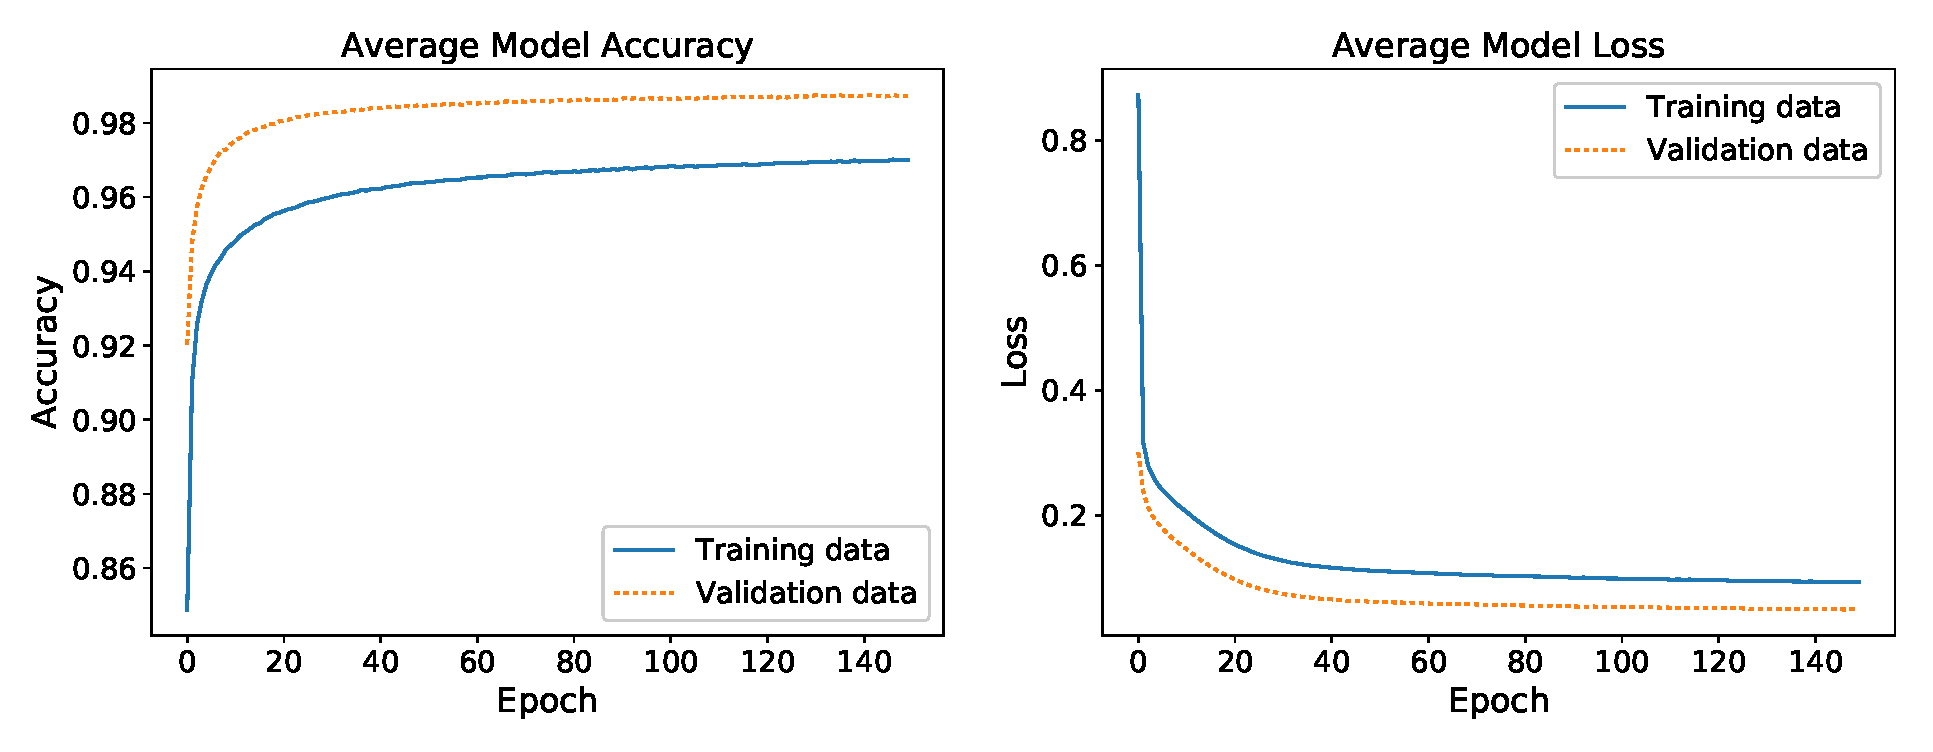
\includegraphics[width=\textwidth]{img/avg_training_metrics}
\caption{Training accuracy and loss progress on training and validation data.}
\label{fig:training_avg}
\end{figure}

To understand how well our model can emulate OSPF we need to analyze the performance on the test set; as we did for the training, we evaluate the performance of the system by averaging the results of the single models. The system achieves an average accuracy of $\textbf{98.71\%}$, with a loss of only $\textbf{0.0496}$; showing really promising results. 
%
With an accuracy of almost $99\%$, LSTM-RNNs performs better than traditional DNNs~\cite{Kato}, which achieves around 90\% of accuracy; however this comparison should be taken with caution, considered that the topologies in the two experiments are slightly different and experiments reproducibility is an open issue in machine learning~\cite{olorisade2017reproducibility}. The comparison of these two approaches is shown in Figure~\ref{fig:lstm_dnn}.

\begin{figure}[b]
\centering
\includegraphics[width=\textwidth]{img/lstm_dnn}
\caption{LSTM and DNN performance comparison.}
\label{fig:lstm_dnn}
\end{figure}

It is important to notice that in this case, the average accuracy could be slightly misleading: the models that represent our model --- a source-destination pair connected by a single link --- are oversimplified, hence it is very likely for them to have an accuracy close to $100\%$. Nonetheless, only $32\%$ (obtained counting all directly connected targets including all the interfaces on the destination router) of the models represents this situation, that means that even if they all had $100\%$ accuracy, the remaining models would have an average accuracy of $97.89\%$.

\section{Overwriting OSPF Routing}
To evaluate our model as OSPF substitution, we observe the behavior of the path prediction system in a functioning network. 
In particular, we  use the same topology (Figure~\ref{fig:topology}) and traffic simulator adopted in the dataset generation phase; to ease the analysis process, all links are set to the same rate. Afterwards, we select a source router and a destination address and examine the difference in behavior between OSPF and our system.

In general, our system shows a dynamic behavior, predicting several paths for the same destination in different traffic conditions. More specifically, we run four traffic simulations, each of them for fifteen minutes, with a varying loss rate on the link chosen by OSPF to connect source and destination;  at the same time, the path prediction system computes a new path every five seconds. The selected target is $(R1, R3)$, with the default path being $R1,R2,R3$ and the loss being varied on the link between R1 and R2. Figure~\ref{fig:path_cmp} compares the routing decisions made by the system in comparisons: being performance unaware, OSPF always chooses the same path, even when the link has losses. Our system on the contrary, shows the ability of behaving dynamically by proposing four alternative paths.

\begin{figure}
\centering
\includegraphics[width=.97\textwidth]{img/path_comparison}
\caption{Routing policies comparison.}
\label{fig:path_cmp}
\end{figure}
By studying the system behavior in presence of losses, it is possible to understand if our model is able to detect and overcome these problems. We test loss rates of 0\%, 5\%,10\%, 15\% and count the number of predictions different from OSPF (table~\ref{tab:same_path_rate}). With the loss set to $0\%$, $43\%$ of the time the predicted path is different from OSPF; if the loss is increased to $5\%$, the ratio of path different from OSPF slightly rises to $45\%$, indicating that the system is able to detect the change. The same happens for a loss of $10\%$, with a much more noticeable improvement in the system behavior;  $63.5\%$ of the proposed paths are in fact, different from the one chosen by OSPF. For the successive loss rate, equals to $15\%$, the performance goes down a little with only a $59.5\%$ different path ratio; the reasons for this loss in performance are discussed in chapter~\ref{ch:conclusion}. The ideal behavior would be for the system to detect the link loss and consequently stop predicting paths going through the damaged link. In our analysis this happens only with a limited loss rate.


Table~\ref{tab:retransmission_rate} compares the resulting retransmission rate of our system, OSPF and Equal Cost Multi Path (ECMP) routing algorithm. The retransmission rate is computed by taking into account how many times traffic would pass through the leaky link, considering two equal-cost paths for ECMP and the ratios in table~\ref{tab:retransmission_rate} for our system. Overall, the system we propose, has a lower retransmission rate than the other strategies, reaching therefore a higher throughput. Figure~\ref{fig:prediction_cmp} is a graphical comparison of the three strategies, showing the time difference needed to transmit the same amount of data. If there is no loss, the three approaches behave the same, however, as soon as a loss rate is introduced, the gap between the curves increases. This increases with the loss rate; however, while it is evident with respect to OSPF, the variation between ECMP and our system is less pronounced.

\begin{table}
\centering
{%
\begin{tabular}{|c|c|c|}
\hline
\multicolumn{1}{|l|}{\textbf{Link loss}} & \multicolumn{1}{l|}{\textbf{Different path rate}} & \multicolumn{1}{l|}{\textbf{Same OSPF path rate}} \\ \hline
0\% & 43\% & 57\% \\ \hline
5\% &45\% & 55\% \\ \hline
10\% & 63.5\% & 36.5\% \\ \hline
15\% & 59.5\% & 40.5\% \\ \hline
\end{tabular}%
}
\caption{Path predictions different and equal to OSPF.}
\label{tab:same_path_rate}
\end{table}

\begin{table}
\centering
\begin{tabular}{|c|c|c|c|c|}
\hline
\multicolumn{1}{|l|}{}  & \multicolumn{4}{c|}{\textbf{Routing Strategy}}                                          \\ \hline
\textbf{Link loss rate} & \textbf{OSPF} & \textbf{ECMP} & \textbf{DNN} &\textbf{LSTM} \\
\hline
0\% & 0\% & 0\% & 0\% & \textbf{0\%}\\
\hline
5\%  & 5\% & \textbf{2.50\%} & 2.70\%	 &2.75\%\\
\hline
10\% & 10\% & 5\% & 7.70\% & \textbf{3.65\%}\\
\hline
15\% & 15\% & 7.50\% & 9\% &\textbf{6.07\%}\\
\hline
\end{tabular}%
\caption{Routing strategies retransmission rate comparison.}
\label{tab:retransmission_rate}
\end{table}

\begin{figure}
\centering
\includegraphics[width=\textwidth]{img/prediction_full_cmp_bar}
\caption{Routing policies retransmission comparison.}
\label{fig:prediction_cmp}
\end{figure}
There is another consideration that needs to be made when talking about OSPF. It would be unfair to consider this protocol completely performance unaware; during our tests, we have noticed that starting from a certain point, OSPF is  able to detect the problem. In our case, with a link loss greater than or equal to $20\%$, OSPF changes its output, selecting a new shortest path. This behavior is caused by the fact that when the loss on the link is too high, the HELLO (i.e., keep-alive) packets used by the protocol are lost, causing the link discovery part of the algorithm to deviate to other routes. We believe that this is a Mininet's limitation and its way to interpret the loss as a fixed phenomenon happening on the link. We know that in real networks losses don't work this way, therefore we are limited in the testing possibilities; nonetheless these results look promising.

\section{A critical scenario}
To have a more clear idea about our system capabilities, we test it in a critical scenario. We decide to simulate a network in which statistically, half of the links are affected by a loss rate; we test the same loss rates of the previous experiments ($5\%$, $10\%$, $15\%$), ten times each, generating traffic between five different targets. The purpose of this experiment is to understand if our system can tolerate better than OSPF a condition where half of the network is not functioning properly. To compare the performance of the two approaches we counted the number of times the links with loss were used; the results are shown in Figure~\ref{fig:stress_test}. The chart compares the total number of defective links traversed in all the runs for each link loss rate. From the results, it appears that our proposed system does not introduce any significant advantage under critical circumstances; the chart shows in fact, that overall, the performance of the two systems are similar, with OSPF performing better when the link loss rate is set to $10\%$ and $15\%$. The reasons of these poor performance are to be found in how our system works: we trained our model to predict alternative paths based on the network conditions; even in this case, the proposed system is able to suggest alternative paths. The main problem is that, given that half of the link in the networks is affected by a loss, the majority of the proposed alternative paths passes through these links, resulting in poor performance. In the conclusions (chapter~\ref{ch:conclusion}) we give a few hints on how to overcome such limitations of our system.

\begin{figure}
\centering
\includegraphics[width=0.949\textwidth]{img/stress_test}
\caption{Comparison of the number of (severely) lossy links traversed by OSPF and LSTM.}
\label{fig:stress_test}
\end{figure}

%!TEX root = tesi.tex
\chapter{Conclusions and Research Directions}\label{ch:conclusion}

In this work, we presented an architecture designed in support of mobile devices task and traffic offloading. Our architecture's aim has been to provide guidelines for task offloading protocol implementations; we prototyped our architecture within a local virtual network testbed based on Mininet.

We focus our attention on a specific traffic offloading policy that leveraged deep learning to predict the best path towards a destination, increasing throughput and reducing perceived latency. Our results showed that despite some limitations, machine learning could be a valid alternative to traditional routing algorithms and can be leveraged to improve network performance. Our results also showed that cooperative routing can steer traffic with better performance than traditional methods, suggesting that applying machine learning in this context is an area worthy of further exploration. 

Our work has some limitations that are not impossible to overcome: we noticed a prediction performance degradation with the increasing loss rate; we believe this is most likely due to our limited training dataset. We also disclose that the quality of our dataset is limited by constraints in both Mininet and the available computation capability. Another problem that needs to be addressed  is the scalability of this approach: training numerous deep learning models requires extensive computational power; being able to reduce the number of models to train would save time and make this system more scalable.

As a future research direction, we suggest analyzing our method with a broader dataset and in different scenarios. Additionally, one could perform a deeper performance analysis by deploying a network that completely replaces OSPF with our system and collects measurements such as throughput and latency. Finally, one could explore more recent machine learning techniques, especially, reinforcement learning, which appear to be promising in solving decision problems.
\nomenclature{\textbf{RNN}}{Recurrent Neural Network}
\nomenclature{\textbf{AI}}{Artificial Intelligence}
\nomenclature{\textbf{ML}}{Machine Learning}
\nomenclature{\textbf{LSTM}}{Long Short-Term Memory}
\nomenclature{\textbf{CNN}}{Convolutional Neural Network}
\nomenclature{\textbf{SDN}}{Software-Defined Networking}
\nomenclature{\textbf{KDN}}{Knowledge-Defined Networking}
\nomenclature{\textbf{OSPF}}{Open Shortest Path First}
\nomenclature{\textbf{ECMP}}{Equal Cost Multi-Path}
\nomenclature{\textbf{DNN}}{Deep Neural Network}
\nomenclature{\textbf{NN}}{Neural Network}
\nomenclature{\textbf{KP}}{Knowledge Plan}
\nomenclature{\textbf{iBGP}}{Internal Gateway Protocol}
\nomenclature{\textbf{BGP}}{Border Gateway Protocol}
\nomenclature{\textbf{eBGP}}{External Protocol}
\nomenclature{\textbf{IP}}{Internet Protocol}
\nomenclature{\textbf{IoT}}{Internet of Things}











%now enable appendix numbering format and include any appendices
\appendix
\include{appendix2}
\chapter{Configure mininet to run the Quagga routing suite}

In the course of these six months of work, I have been slowed down by numerous issues that came up as my reasearch was proceeding; these issues were due to my inexperience with the software and its complexity. To implement the deep learning model, I needed a functional network with running routing algorithms. At first the solution looked simple, I just had to run the Quagga routing suite on the mininet nodes. Accomplishing this result took me away a lot of time, so I have decided to highlight here the problems I have faced. Here's the list:
\begin{itemize}
\item by default, mininet doesn't support loops in a topology: if you want to have a complex closed topology you need to manually enable the spanning tree protcol on every switch
\item when you build Quagga from source, the link to the dynamic libraries are not automatically created, to solve the problem run:
\begin{lstlisting}
sudo ldconfig
\end{lstlisting}
\item the Quagga service config in mininext relies on init.d scripts which are not installed when you build it from source, the quickest solution is to install quagga from the distribution repositories
\item in mininet, the default ovs-controller doesn't support more than sixteen switches; if you need a bigger network you need to install the mininet patched version of the openflow controller (\url{https://github.com/mininet/mininet/wiki/FAQ#ovs-controller})
\item in miniNext, it is not possible to capture traffic directly on the hosts (in my case quagga routers) because they’re in a different namespace. The workaround is to set up a switch on every link (between each pair of routers) and analyze the traffic on its interfaces; for the problem described in the previous point, the number of switch limits the network size
\item ryu is not able to talk with the mininet switches that do not have the canonical name (s1, s2, ...)
\item the output of OSPF depends on the nominal speed interface declared in the Zebra configuration file, changing the link speed through mininet doesn't affect the algorithm
\end{itemize}

%next line adds the Bibliography to the contents page
\addcontentsline{toc}{chapter}{Bibliography}
%uncomment next line to change bibliography name to references
%\renewcommand{\bibname}{References}
\bibliography{refs}        %use a bibtex bibliography file refs.bib
%\bibliographystyle{plain}  %use the plain bibliography style
%\bibliographystyle{abbrvnat}
\cleardoublepage
\end{document}

